\chapter{Platform Design}
This chapter contains the details of physically a quadcopter for use in a confined space. The hardware design decisions are preceded by giving an overview of the total system design. After the high level design has been done, this chapter looks into different platform designs and rotor configurations. Based on analysis of empirical data and knowledge learnt through an analysis of conventional rotors in Section \ref{SECT_RotorConfig}, the best suited rotor configuration is identified. Once a suitable platform has been chosen, a look into the required electronics is done. This includes all the electronics required for stable flight, as well as sensor requirements for operations and flight strategy. The chapter is concluded with a summary of the platform decisions made and used in the simulation.

The final design will be modelled and used to validate the proposed outcomes for this work. Although this chapter will discuss the various aspects of a quadrotor, it will focus on the components required for creating an accurate simulation of the system.

	\section{System Hardware Architecture}
	The following section gives an overview behind the system design of \projectName. The section begins by working through the hardware system architecture shown in Figure \ref{IM_SystemArchitecture} and identifying the objectives and roles of each subsystem in the design. The first consideration is the size and mounting needs of the system, provided by the mechanical platform. This gives a good start to elaborate on the needed capabilities of the proposed method of propulsion. The next considerations are the electronic modules required to run all the necessary peripherals and obtain all the required sensor data.
	
	The system architecture for \projectName is laid out below in Figure \ref{IM_SystemArchitecture}. The hardware system comprises of 3 main subsystems, namely Mechanical Construction, Propulsion and Electronics. The role each subsystem plays in meeting the system requirements is discussed in more detail below.
	
	\begin{figure}[H]
		\centering
		\includegraphics[height = 15cm]{../Design/System/SystemArchitecture/SystemArchitecture.jpg}
		\caption{System Architecture}
		\label{IM_SystemArchitecture}
	\end{figure}

		\subsection{Platform Construction}
		The platform is the physical embodiment of the craft. In this context this includes the mechanical construction of the craft, as well as the flight generating components.
		
			\subsubsection{Mechanical Construction}
			The mechanical construction of the system introduces size and weight restrictions for the rest of the system. It should provide adequate mounting for the necessary peripherals described in the sections following, while remaining as light weight as possible. The structure needs to protect the rotors from collisions by means of a protective shroud and include lightweight landing gear. The chassis must also be such that the weight is distributed as symmetrically as possible. The propulsion system must be housed and provided with rigidity for steady flight control.
			
			\subsubsection{Propulsion and Flight Characteristics}
			The propulsion system comprises of the motors and propellers. This subsystem needs to supply enough thrust and overhead for steady control, as well as enough lifting capacity to carry any additional, mission sensors. The craft should be able to handle an external sensor payload. To ensure capable disturbance rejection, the total maximum thrust should include sufficient overhead above the hover requirement.
			
			The craft must efficiently hover and fly at low speeds. The craft should have multiple control surfaces to accurately counter disturbances. Due to the intended use case in narrow corridors, the craft will fly with a set orientation and thus does not require the abilities for sharp turns of manoeuvres.	
		
		\subsection{Electronics Interface}
		At the core of any reliable robotic platform is a thoroughly planned electronics system, for \projectName this is the most complex subsystem containing the most modules. It is responsible for all intelligence and power generation. This section breaks this subsystem into more discrete parts. It begins by separating the two computing modules into real time and non-real time components. The real time components include some of the on board sensors which are required for stable and fast control, which all feed into the flight controller. For the drone to successfully autonomously navigate an environment, it will need to better understand it's surroundings. The flight controller will analyse this data and based on flight software will control the electronic speed controllers (ESCs). The on board computer (OBC) will process and handle all non flight critical sensor information and can be considered as the mission computer. The OBC must also have provision to connect to a sensor pack via a predetermined interface. Another useful and necessary function, will be the ability to illuminate a dark area. 
		
		The network design will also consist of 2 discrete wireless links. Each link is dedicated to one of the computing modules. The real time node will be interfaced through a low bandwidth, high range and high reliability interface. With the non-real time node linking to the high bandwidth interface which will have lower range and reliability requirements. Both of these interfaces will link to a ground station of some sort.
		
		No system can operate without a sufficient power source. In the case of any robotic system it is important that every aspect of the design is optimised. The capacity of the power supply is limited by weight and should be optimised to the lifting capacity of the platform. Once the battery chemistry has been decided upon, work can be done to design a robust power management system. Limiting the leakage of every subsystem as well as choosing efficient modules are both part of an effective power management system. The analysis of the power system is important since it generally contributes a very high percentage to the overall mass of the craft.
		
			\subsubsection{Flight Controller}
			The flight controller is responsible for handling all the flight critical sensor data. Using a motor mixing algorithm the flight controller will then output signals to the electronic speed controllers. There are multiple options for flight controllers, all tailored to different applications, platforms and flying styles; each option has their own level of reconfigurability. For this application it is important that the chosen flight controller allows access to both the inner control loops as well as allows additional sensor data to be added into the architecture. The flight controller is also responsible for handling the pilot commands and waypoints sent via the radio link, as well as transmitting in flight diagnostic information back to the ground control station.
			
			The flight controller's computing time capabilities have a direct influence on the system. This timing needs to be understood and introduces requirements on the controller designs. Any additional computing the craft needs should be handled by the OBC and not the flight controller. This will reduce the risk of unmodelled timing delays and unrealistic controller design goals.
			
			\subsubsection{Electronic Speed Controller}
			The above mentioned flight controller sends a motor control command to the electronic speed controller (ESC). The ESCs then in turn directly control the speed of each motor. Each motor should have a dedicated ESC. This part needs to be chosen based on the maximum amount of current it can handle. At $100$\,\% throttle the current draw of the motor should not exceed $75$\,\% of the ESC's limit. Another important consideration is the ESC's refresh rate and computing speed. The flight controller will be rapidly sending data to the ESC. The quicker the module can respond, the more robustly the platform will be controlled. Possible timing delays can be accounted for by ensuring the controllers have sufficient phase margins. 
			
			\subsubsection{On Board Computer}
			Where the flight controller ensures the craft maintains steady flight, the On Board Computer (OBC) handles all higher level processing and flight strategy. This will include interfacing to the rest of the on board sensors, the sensor pack as well as handling the high bandwidth networking to the ground station. The OBC should not be required for flight purposes, and can thus be considered as a dedicated mission computer. 
			The OBC should be as light weight and low power as possible while being sufficiently powerful to do real time analysis of camera data for future missions. The OBC must have multiple standard communication ports to easily interface to other sensors. There should also be a highly reliable, and fast interface between the OBC and the flight controller, thus allowing more complex flight strategies to be put in place, while not risking the robustness of the tracking control.
		
			\subsubsection{On Board Sensors}
			The on board sensors can be split up into two distinct categories. The first set of sensors are to enable stable flight of the craft and are used to close the control loops. Examples of such sensors would be inertial measurement units (IMU), global positioning units (GPS) and other relative velocity measuring sensors. 
			
			The second set of on board sensors are required for enabling more intelligent autonomous flying strategies. Examples of these sensors include proximity measurements to enable obstacle avoidance and localisation. Other types of sensors from this set could include condition monitoring of the craft's batteries. 
		
			\subsubsection{Sensor Pack}
			The actual sensor pack in question will remain generic. So that the platform can cater for an array of sensing devices and applications. To ensure compatibility, the sensor pack needs to be powered and communicated to. It will have access to interface directly to the OBC. Typical examples of sensor pack application would be mapping equipment and stored video feed for post flight inspections.
		
	\section{Platform Construction}			
		\subsection{Design Considerations}
		Before a proper analysis can be done, specific design criteria need to be outlined; this includes parameters such as the required flight time and manoeuvring decisions.

			\subsubsection{Physical Restrictions and Requirements}
			One of the major components \projectName will have to overcome is to navigate these unknown areas and not only survive collisions, but also reject the disturbances introduced by being close to the walls. Since mine shafts are predominantly long and narrow, the same approach will be looked at for the design of the drone. To optimise the size of rotors that can be used the platform will also be designed to be long and narrow. 
			Since the drone will be required to navigate very confined spaces, the smaller the drone the better. The minimum size of the drone is limited by the need for adequate flight time as well as payload capacities which require a higher disk loading.
			
			\subsubsection{Manoeuvring Decisions}
			The manoeuvring decisions are dependant on the type of environment and type of missions required by the platform. These decisions influence the final design of the craft.
			The end use case for \projectName will include mapping of unknown areas. To complete this, it will simplify the procedure if the drone keeps it's orientation during flight. Due to the nature of the environment, fast speeds will not be used regularly. Therefore \projectName will be designed to have slow, steady and controlled movements.
			
			\subsubsection{Disturbances}
			Apart from the difficulty of navigating and manoeuvring through an unmapped area there are other disturbances introduced into the system. Some common disturbances found were outlied in Section \ref{SSECT_Disturbances}.
			Due to the nature of the tunnels, wind gusts are created that funnel through these passageways. These winds will produce large undesired drag moments and forces.
			The effect of coming close to a wall or floor has been discussed in the literature study. Since the areas will be unknown and complex, collisions and bumps are extremely likely. The flight strategy will try and ensure the drone does not collide with the environment. However, the drone must be able to withstand a collision and maintain it's orientation as best as possible.
			
			\subsubsection{Thrust Overhead}
			The total overhead of a rotorcraft is a percentage above the thrust required for hover. This value determines a craft's ability to manoeuvre, with a higher value giving it more freedom and a greater ability to resist disturbances. With these benefits the system does become very sensitive and more difficult to control and stabilise. Since the craft will be in confined narrow passages, the craft does not need to be fast moving. Rather a "slow and steady" pace will be approached. The craft does however need enough power to counteract the disturbances described above. These considerations lead to a value of $150\%$, with $100\%$ being enough thrust to hover.
			
			\subsubsection{Flight Time}
			Flight time is dependant on efficiency and power requirements of the system as well as the capacity of the on-board power source. This becomes a typical optimisation problem. By adding a larger power source the weight is increased and therefore the platform requires more power to keep itself aloft. Weight is a determining factor for any aerial system and influences flight time, for this reason the weight of every subsystem must be optimised. To ensure the craft can complete a mission it will need sufficient flight time. Initial discussions have set 30 minutes as the bottom limit. The original platform might not be able to reach this goal, but once the platform is performing adequately adjustments can be made to the system to optimise weight and power consumption. 
			
		\subsection{Chosen Concepts}
		The traditional configurations of drones struggle to handle disturbances introduced by being in a confined space. Traditional configurations are also not optimised for fitting inside a long narrow space. For these reasons a few unique designs were considered and are discussed below.
		For the comparison, it was assumed that thrust to RPM and RPM to current are linear relationships.
		
		Two concepts were selected as final candidates. This next section walks through some of the important factors considered and ultimately, why certain decisions were made. The naming convention used is shown in Figure \ref{IM_UnlikeSizes}.
		On the left of Figure \ref{IM_UnlikeSizes} represents the \textit{"Unlike Size Quad"} and the right of Figure \ref{IM_UnlikeSizes} is the \textit{"Overlapping Quad"}. 
		\begin{figure}[H]
		\centering
		\includegraphics[height = 6cm]{Images/Design/UnlikeSizes}
		\includegraphics[height = 6cm]{Images/Design/Overlapping}
		\caption{Rendering of initial concept of the unlike rotor size quadcopter (Left). Malloy Aeronautics Hoverbike Concept (Right) (Picture taken \cite{MAHover}).}
		\label{IM_UnlikeSizes}
		\end{figure}
			
			\subsubsection{Concept 1 - The Overlapping Quad}
			The overlapping quad is a concept pursued by Malloy Aeronautics \cite{MAHover}. They used the design in an initial concept of their hover bike personnel carrier, which requires a large payload capacity. The design uses an H-formation for it's rotors, except the rotors are brought in to limit the width of the craft to the point that they overlap, as shown in Figure \ref{IM_UnlikeSizes}. Each overlapping pair will have both spin directions, this feature is shown in Figure \ref{IM_OverlappingPair}.
		
			\begin{figure}[H]
			\centering
			\includegraphics[height = 6cm]{Images/Design/OverlappingVD}
			\caption{Overlapping concept, visual representation of rotor pairs. Image modified from \cite{MAHover}}
			\label{IM_OverlappingPair}
			\end{figure}
			
			Overlapping rotors introduce an inefficiency into the system. Figure \ref{IM_SeperationGraph} illustrates how the percentage overlap affects the total efficiency of the rotors.
			
			\begin{figure}[H]
			\centering
			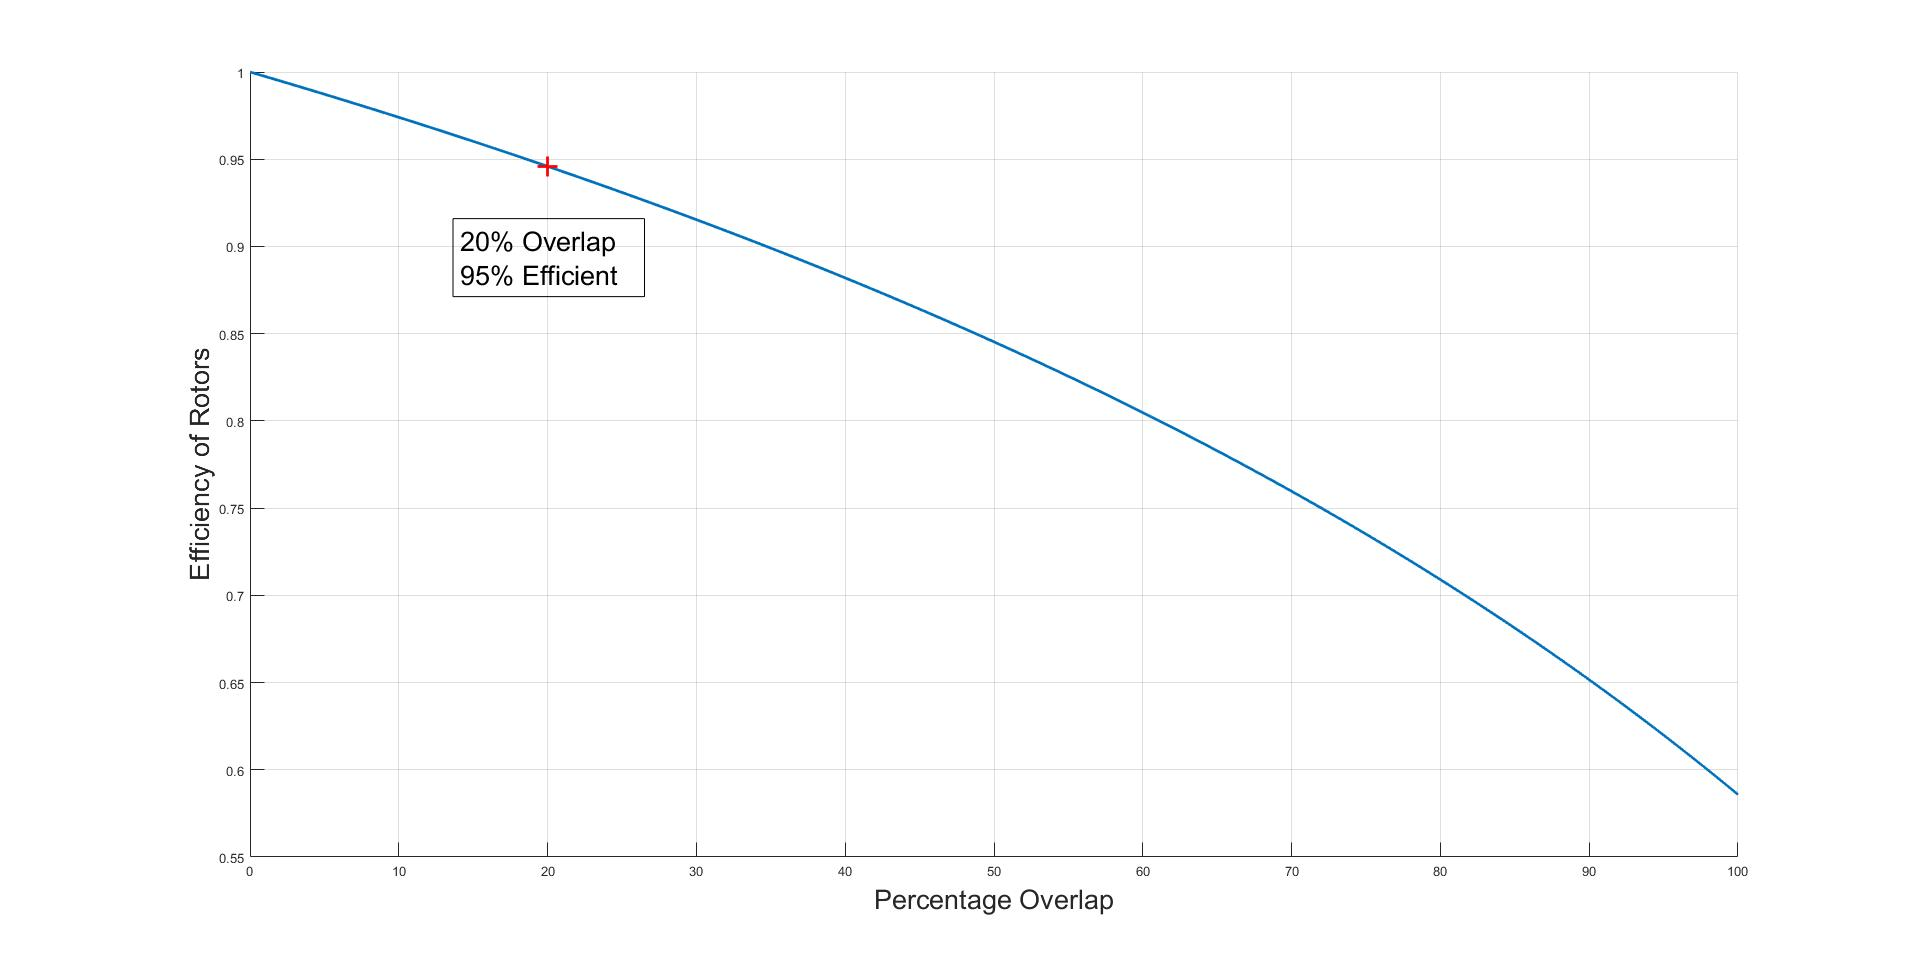
\includegraphics[height = 7.9cm]{Images/RotorOverlap.jpg}
			\caption{Graph representing the effects of overlapping rotors in a quadrotor}
			\label{IM_SeperationGraph}
			\end{figure}
			
			A large benefit to this design is the power to size ratio. This benefit can be utilised through handling larger payloads, or a larger battery pack increasing total flight time.

			\subsubsection{Concept 2 - The Unlike Size Quad}
			The unlike size quad is an original design that uses the standard cross formation, except it has two pairs of different size rotors. This means that the counter rotating pairs will be set up as shown in Figure \ref{IM_UnlikeSizePair}, with each rotation direction having one big and one small rotor. 
			
			To maintain a common disk loading in the system, the thrust requirement will be lower on the smaller blades and larger on the bigger blade. The smaller the side rotors get, the higher the thrust requirements of the larger rotors become, this limits the rotor size ratio. Initial calculations, factoring in thrust overhead, overall size of the craft and minimum thrust allowed to rotors, set the ratio between $65\% - 80\%$.  When approaching the lower bound, the thrust requirement for hover alone leaves very little room for manoeuvring or disturbance rejection. The upper bound reaches a point where the size difference is so negligible the design's narrow intent is lost.
			
			\begin{figure}[H]
			\centering
			\includegraphics[height = 6cm]{Images/Design/UnlikeSizeRotorPair}
			\caption{Unlike Size Quad visual representation of rotor pairs}
			\label{IM_UnlikeSizePair}
			\end{figure}
			
			The second important choice is how far to put the rotors away from the centre. As the craft gains translational speed, the air doesn't come in directly from the top any more as shown in \ref{IM_MomentumTheoryAirFlow}. Instead it now starts to come in at an angle. As the craft then manoeuvres and changes it's orientation, the air starts coming in at more extreme angles. If the electronics housing has a lot of height it can interfere with the wake boundary and create an inefficiency. This inefficiency is also based on how far the rotors are from the housing. Therefore, before this decision can be made the limits of how small the centre electronics housing needs to be decided. 
			
			Through discussions and observations of current systems a minimum limit of $75mm \times 75mm$ was set. To avoid overlap, the distance from the centre of the big rotor and the centre of the craft will be at the very least $R$. Including space for the housing increases this.
			
			Since the craft needs to remain narrow, the side rotors can be brought in as well as shrunk. This would require pushing the two larger rotors slightly more out. Bringing the side rotors in closer to the middle housing will reduce efficiency, so a compromise must be chosen between width and efficiency. Since the side rotors don't contribute as much to the system as their bigger counterparts, they have the option of a lower separation distance. The lower separation distance can also be justified by the lower need and use of roll moments and side translations.
	
		\subsection{Concept Comparison}
		The comparison of the two concepts includes hover efficiency, thrust, electrical power requirements, size and manoeuvrability. The final decision will need to be made with certain assumptions in mind. These assumptions as well as the method of comparison are described below. 
	
			\subsubsection{Assumptions and Method}
			Since both designs use 4 rotors they can be compared relative to a well known design, the standard quadrotor. For each configuration certain parameters need to be decided before a comparison can be done. 
			
			If hover is a thrust of $100\%$, the overhead was set at $50\%$ of that, to a total of $150\%$. The mass in question includes provision for a sensor pack of undecided mass. 
			
			The unlike size quad had it's small rotors set at $75\%$ of the larger ones, this decision is explained further in the text. To give a quantifiable reference, R was set at $254mm$. With that assumption the unlike size quad moves it's side rotors in to a distance of $300mm$ and the larger rotors were moved to $508mm = 2R$ away. The overlapping quad set a separation distance of $350mm$ which created an overlap factor of $20\%$. 
	
			\subsubsection{Rotor Area}
			If a rotor size of $R$ is assumed for the rotors\footnote{The big rotors in the case of the unlike size quad} then the total area for a standard quad will be $A_{std} = 4 \pi R^2$. The reduction in radius of the two smaller rotors leads of the unlike size quad leads to a decrease in area of  $78.13\% of A_{std}$. 
			
			\subsubsection{Thrust and Power Considerations}
			The decision to set the smaller rotors to $75\%$ was based on observation of thrust ratios between the rotors. The final value of thrust required from each rotor as a percentage is shown in Figure \ref{IM_ExcelGraphs}. The points marked are at minimum, hover and maximum. The total thrust available to the unlike size quad is $\approx 78\%$ of the thrust available to the standard design. This reduced value also comes at a weight reduction. The overlapping quad has an equal total rotor area but an inefficiency is introduced by the overlap as according to \eqref{EQ_OverlapEfficiency}. Therefore the overlapping quad has $95\%$ of the total thrust capacity, without the weight reduction.
			
			\begin{figure}[H]
			\centering
			\includegraphics[height = 10cm]{Images/Design/ExcelGraphs}
			\caption{Graphical representations of the thrust ratios for the unlike size quad}
			\label{IM_ExcelGraphs}
			\end{figure}
			
			The values for electrical power were calculated according to how much energy would be needed to obtain the same thrust as the standard design. The inefficiency introduced by the overlap relates to a reduction in thrust of $\Delta T_{overlap} = 5.36\%$, therefore $\Delta P_{overlap} = 14.21\%$ is needed to overcome this loss, based on \eqref{EQ_ElectricalPowerThrust}. 
			
			For the unlike size quad, the reduction in rotor size leads to a substantial loss in aerodynamic power, even with a small reduction in inertia. To regain that power, the rotors need to be pushed harder, this leads to an increase in electrical power. A value of $\Delta P_{unlike size} = 18.5\%$ is be calculated.
	
			\subsubsection{Size and Manoeuvrability}
			The size was calculated as though the drone made a rectangular box and with the rough values above, Table \ref{TAB_SizeComparison} puts those values in a tabular format.
			
			\begin{table}[H]
				\centering
				\begin{tabular}{l | c | c }
					Concept & Length ($mm$) & Breadth ($mm$) \\
					\hline\hline
					Unlike Size	   	& 1524 & 981 \\
					Overlapping    & \boldmath$1308$ & \boldmath$858$ \\
					Standard		& 1524 & 1524\\
				\end{tabular}
				\label{TAB_SizeComparison}
				\caption{Table representing the size comparison of the two concepts}
			\end{table}
			
			As shown both crafts are similar in size, with the overlapping design being slightly shorter as well as more narrow.
			
			\subsubsection{Discussion}
			The quantifiable values are culminated below in Table \ref{TAB_ConceptComparison}. The winner of each parameter is written in bold.
			
			\begin{table}[H]
				\centering
				\begin{tabular}{l | c | c | c | c | c }
					Concept & Disk Loading & Total Thrust & Electrical Power & Length ($mm$)& Width ($mm$) \\
					\hline\hline
					Unlike Size	  & \boldmath$78.13\%$  & $78.13\%$ 	& $118.57\%$	& $1524$ & $981$ \\
					Overlapping    & $80.18\%$ & \boldmath$94.64\%$  & \boldmath$114.21\%$	& \boldmath$1308$ & \boldmath$858$ \\
					\hline\hline
					Standard		& $100\%$ 	& $100\%$  	  & $100\%$			& $1524$ & $1524$\\
				\end{tabular}
				\label{TAB_ConceptComparison}
				\caption{Table representing the end comparison of the two concepts}
			\end{table}
			
			The overlapping quadrotor introduces a significant size reduction to the standard quadrotor while losing minimal thrust to inefficiencies. This allows for a larger more powerful drone to be deployed in tight spaces. The extra required electrical power can be nullified by the ability to carry a larger power source thus increasing flight time.
			
			Malloy Aeronautics sell what is called a \textit{Drone-3 Kit}, it includes various accessories to help developers use the platform.	Based on the above analysis and conclusions the overlapping quadrotor design will be used as the design going forward.

	\section{Electronic Design}
	At the core of any reliable system is a thoroughly planned electronics system. There are multiple aspects this subsystem must handle. Due to the rapidly increasing market and interest in multirotors there has been a wave of developers and designers creating devices for these specific purposes. The first and foremost is monitoring and controlling flight dynamics.	
	
	The on board computer will handle the data streams and control the non-real time peripherals. For the drone to successfully navigate an environment it will need to better understand it's surroundings. To achieve successful navigation, a few onboard sensors have been looked at. Another design consideration is the provision for a sensor pack. This section of the study will also involve looking at potential external sensors and providing accessibility for them.
	
		\subsection{Flight Controller}
		There are multiple options for flight controllers, all tailored to different applications and flying styles. This section identifies some possible options
		
			\subsubsection{Custom Design}
			Given the time and resources most final products will look at custom designing some hardware and electronics. The benefits of custom design include complete control over the operation and functionality of the design as well as reduced cost when scaling up. The development of a custom design however can be very taxing and costly.
			
			It is also common for a research lab to dedicate time into developing such modules. By using MITs custom board, Cutler in his masters dissertation demonstrates this \cite{How2012}. \textit{The University of Stellenbosch's Electronics System Lab} produced a custom design in \todo{insert date the boards were designed and reason we're not using them}. This board is under redesign and unfortunately cannot be used for this project.
		
			\subsubsection{Pixhawk}
			The need for a commercial solution becomes evident. Due to the growing hobbyist community, some flight controllers are difficult to modify and are designed for use as a \textit{"plug and play"} module. Fortunately there is also a large designer community which has created the need for more configurable modules.
			
			Figure \ref{IM_Pixhawk} shows the \textit{Pixhawk}, which is marketed as an autopilot module for fixed wing and rotor wing aircraft. It is specifically tailored for research and is listed as open-hardware\footnote{https://store.3dr.com/products/3dr-pixhawk}. Due to the open platform it has created an experienced community with good documentation and other forms of assistance.
			
			\begin{figure}[H]
				\centering
				\includegraphics[height = 6cm]{Images/System/Pixhawk.jpg}     
				\caption{Pixhawk Flight Controller}
				\label{IM_Pixhawk}
			\end{figure}
			
			It features a 32 bit STM32F427 processor, running at 168MHz with 256Kb of RAM and 2Mb of Flash memory. It comes equipped with a full inertial measurement unit (IMU), consisting of a gyroscope, accelerometer and magnetometer. The Pixhawk also includes an integrated barometer and has an additional 32 bit co-processor that acts as a failsafe. There are multiple interfacing capabilities as well as a built in power protection unit\footnote{https://pixhawk.org/modules/pixhawk}. 
			
			The Pixhawk has been designed for robotic applications thus is light weight and power efficient. It operates on a real time operating system called \textit{NuttX} which has Unix characteristics but is much lighter than a different operating system such as Linux. This provides a lot of reconfigurability which is needed in this project.
		
	
		\subsection{On Board Computer}
		The On Board Computer (OBC) is required to handle all higher level processing. In an aerial application weight and power consumption are both important considerations. Based on current available commercial products a few were selected. The advantages and disadvantages of each are described below.
	
			\subsubsection{Raspberry Pi 3 Model B}
			
			The Raspberry Pi has become a well known and respected piece of hardware. It has generated a large community and thus resources are readily available and the device can be bought locally. The new version of the device runs a 1.2GHz 64-bit quad-core ARMv8 CPU and includes built in Bluetooth and WiFi modules, an image from the Raspberyy Pi website is shown in Figure \ref{IM_Pi}\footnote{https://www.raspberrypi.org/products/raspberry-pi-3-model-b/}. 
			
			\begin{figure}[H]
				\centering
				\includegraphics[height = 6cm]{Images/System/Pi.jpg}     
				\caption{Raspberry Pi 3 Model B}
				\label{IM_Pi}
			\end{figure}
			
			It has a large 40 pin GPIO connector, 4 USB connections and an Ethernet port. The Pi's main advantage would be the access to the online community constantly updating Raspberry Pi resources and forums. With the community also comes example projects and large variety of compatible hardware and open source software. With a maximum current of 2.5A at 5V, the 12.5W computer is relatively low powered which suits this application. However there are more powerful machines that can run more intense algorithms at the cost of more power.
	
			\subsubsection{Odroid XU4}
			Hardkernel has designed a compact high processing power unit called the Odroid XU4. It has gained respect in some developer communities due to it's incredible processing power. It can run both Android, Ubuntu and other similar Linux based operating systems. Hardkernel has generated an immense of documentation and wiki pages, all available on their website\footnote{http://www.hardkernel.com/}. They also have a team of developers creating new devices to interface with the devices. 
			
			\begin{figure}[H]
				\centering
				\includegraphics[height = 6cm]{Images/System/XU4.jpg}     
				\caption{The Odroid XU4}
				\label{IM_Odroid}
			\end{figure}
			
			The XU4 hosts a Samsung Exynos5422 Cortex™-A15 processor running at a 2GHz clock speed and an additional Cortex™-A7 Octa core processing unit. This allows for incredible processing capabilities and speed, an image from Hardkernel's Website is shown in Figure \ref{IM_Odroid}. The rated power supply for the unit is a 4A at 5V module. Including a 20W module on board will add a significant drain on the power source. It comes with 2 stable USB 3.0 ports and an additional USB 2.0 connection. 
			
			The Odroid is also frequently used at the CSIR, opening up experience and knowledge on the devices.
		
		
		\subsection{Location}
		An important part of any robotic application is localisation. As stated earlier, an underground environment limits the use of traditional GPS. Stellenbosch University as well as the CSIR are both funding research into localisation in a GPS constraint environment. Until such a time that these technologies are readily available, this project will work with traditional GPS devices.
		
		As discussed previously, this project will not be designing for a GPS constraint environment. Fortunately there are many commercial  GPS modules available for purchase. Each with their own advantages and disadvantages. For this project the module needs to be lightweight and low power. The GPS needs to create speed and translation data, this information is crucial when generating maps of unknown areas. The PixHawk website recommends the 3DR uBlox GPS kit\footnote{https://store.3dr.com/products/3dr-gps-ublox-with-compass}. Although many alternatives exist, the open source hardware status creates ease of integration and support. With these considerations, this module has been chosen.
		
		It weighs a total of 16.8gs and as has a low 8.5mm profile. This module will perform adequately and fulfil the design needs of the project.
	
		\subsection{Object Avoidance}\label{SECT_ObjectAvoidance}
		Due to the nature of the project, object avoidance is an important attribute to include in the design. Obstacle avoidance requires that the drone has some level of an understanding of the environment. This information can then be used in higher processing nodes to actively avoid objects and plan routes. A few different sensor options are observed below, each with a set of advantages and disadvantages. 
		
			\subsubsection{Laser Range Finders}
			Laser range finders can be found in a multitude of high end robotic platforms often in the form of a Lidar. They exhibit high accuracy and can be bought as full $360$\textdegree modules. Lidars are expensive and heavy making them less suitable for this application.
			
			\subsubsection{Ultrasonic Proximity Sensors}
			Ultrasonic sensors are already used in aircraft, generally as downward facing to accurately predict altitude. Relatively speaking ultrasonic sensors are cheap and light weight and consume little power. They are however prone to measurement errors when used against non-uniform surfaces and require additional processing to ensure that multiple sensors do not influence each other. These sensors produce a measurement cone, rather than a directed pinpoint measurement providing a large coverage area per sensor. For this work ultrasonic proximity measurement will be used.
			
			
			
	